\documentclass[border=6pt]{standalone}
\usepackage{amsmath}
\usepackage{tikz}
\usetikzlibrary{positioning, arrows.meta, fit, backgrounds, calc}
\tikzset{stage/.style={draw, rounded corners, align=center, font=\small, minimum height=1.0cm, minimum width=2.6cm, thick},layer/.style={draw, dashed, rounded corners, inner sep=10pt},node_t/.style={draw, circle, align=center, font=\scriptsize, minimum size=1.0cm, thick},flow/.style={-{Stealth[length=2.5mm]}, thick},edge_t/.style={-{Stealth[length=2mm]}, font=\scriptsize}}
\begin{document}
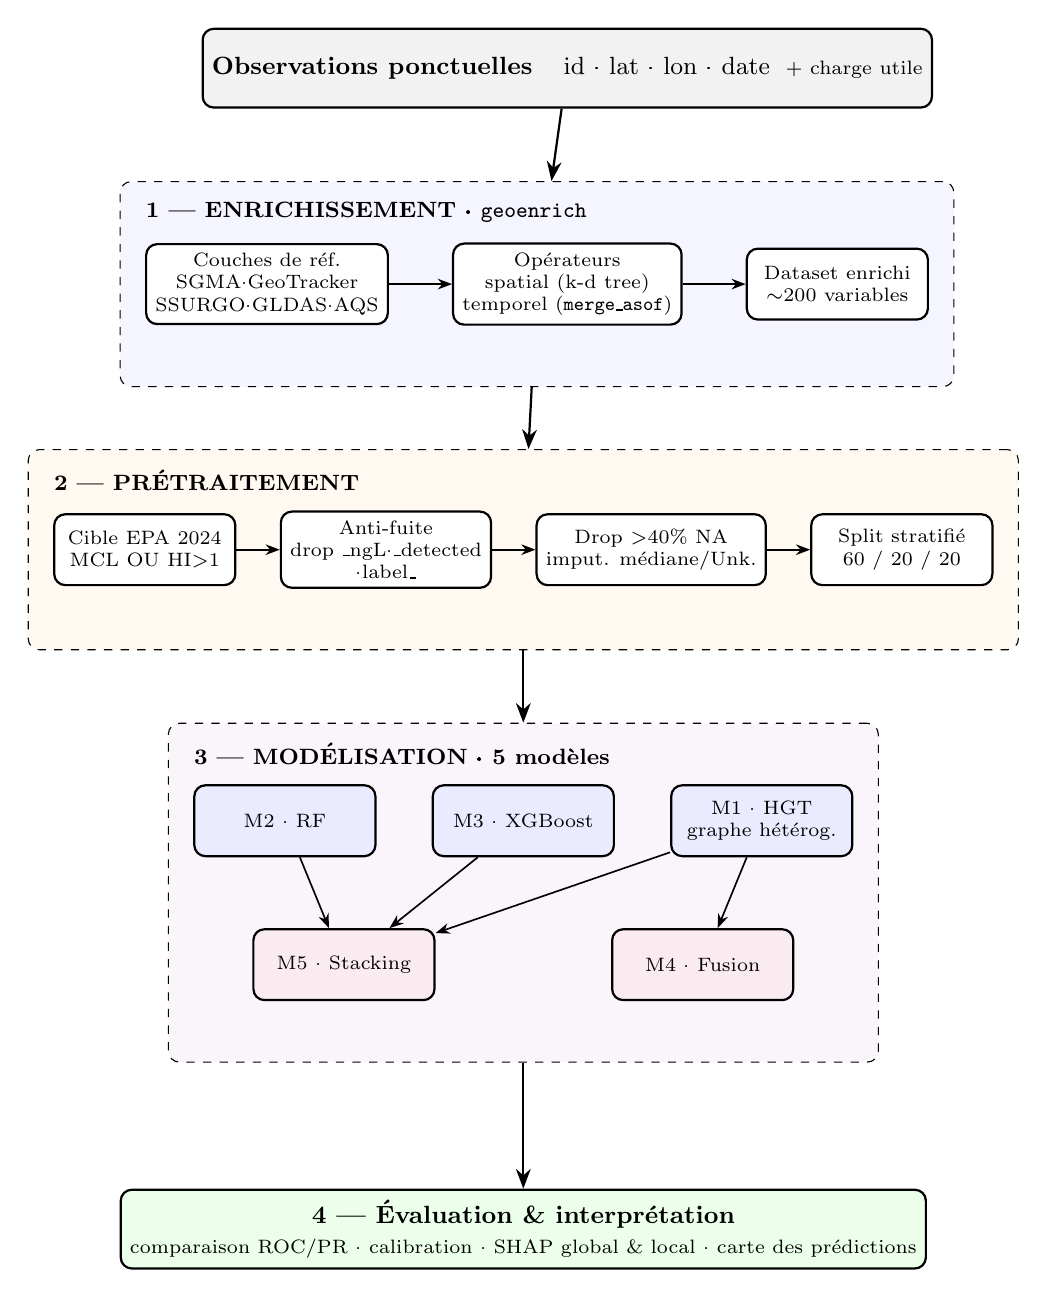
\begin{tikzpicture}[
   sub/.style={draw, rounded corners, align=center, font=\scriptsize,
               minimum height=0.9cm, minimum width=2.3cm, fill=white, thick},
   big/.style={draw, dashed, rounded corners, inner sep=9pt, inner ysep=22pt},
   sflow/.style={-{Stealth[length=1.8mm]}, semithick}]

  % Observations
  \node[stage, fill=gray!10, minimum width=8cm] (obs)
    {\textbf{Observations ponctuelles} \;\; id · lat · lon · date \;{\scriptsize+ charge utile}};

  % 1. Enrichissement
  \node[sub, below=1.7cm of obs] (oper) {Opérateurs\\ spatial (k-d tree)\\ temporel (\texttt{merge\_asof})};
  \node[sub, left=0.8cm of oper] (ref) {Couches de réf.\\ SGMA·GeoTracker\\ SSURGO·GLDAS·AQS};
  \node[sub, right=0.8cm of oper] (enr) {Dataset enrichi\\ {\scriptsize$\sim$200 variables}};
  \draw[sflow] (ref) -- (oper); \draw[sflow] (oper) -- (enr);
  \begin{scope}[on background layer]
    \node[big, fill=blue!4, fit=(ref)(oper)(enr)] (s1) {};
  \end{scope}
  \node[font=\footnotesize\bfseries, anchor=north west] at ([xshift=6pt,yshift=-4pt]s1.north west)
    {1 — ENRICHISSEMENT · \texttt{geoenrich}};

  % 2. Prétraitement
  \node[sub, below=1.6cm of s1, xshift=1.45cm] (na) {Drop $>$40\% NA\\ imput. médiane/Unk.};
  \node[sub, left=0.55cm of na] (leak) {Anti-fuite\\ drop \_ngL·\_detected\\ ·label\_};
  \node[sub, left=0.55cm of leak] (tgt) {Cible EPA 2024\\ MCL OU HI$>$1};
  \node[sub, right=0.55cm of na] (spl) {Split stratifié\\ 60 / 20 / 20};
  \draw[sflow] (tgt) -- (leak); \draw[sflow] (leak) -- (na); \draw[sflow] (na) -- (spl);
  \begin{scope}[on background layer]
    \node[big, fill=orange!5, fit=(tgt)(leak)(na)(spl)] (s2) {};
  \end{scope}
  \node[font=\footnotesize\bfseries, anchor=north west] at ([xshift=6pt,yshift=-4pt]s2.north west)
    {2 — PRÉTRAITEMENT};

  % 3. Modélisation
  \node[sub, fill=blue!8, below=1.7cm of s2] (xgb) {M3 · XGBoost};
  \node[sub, fill=blue!8, left=0.7cm of xgb] (rf) {M2 · RF};
  \node[sub, fill=blue!8, right=0.7cm of xgb] (hgt) {M1 · HGT\\ graphe hétérog.};
  \node[sub, fill=purple!8, below=0.9cm of rf, xshift=0.75cm] (stk) {M5 · Stacking};
  \node[sub, fill=purple!8, below=0.9cm of hgt, xshift=-0.75cm] (fus) {M4 · Fusion};
  \draw[sflow] (rf) -- (stk); \draw[sflow] (xgb) -- (stk); \draw[sflow] (hgt) -- (stk);
  \draw[sflow] (hgt) -- (fus);
  \begin{scope}[on background layer]
    \node[big, fill=violet!4, fit=(rf)(xgb)(hgt)(stk)(fus)] (s3) {};
  \end{scope}
  \node[font=\footnotesize\bfseries, anchor=north west] at ([xshift=6pt,yshift=-4pt]s3.north west)
    {3 — MODÉLISATION · 5 modèles};

  % 4. Évaluation
  \node[stage, fill=green!8, below=1.6cm of s3, minimum width=9cm] (eval)
    {\textbf{4 — Évaluation \& interprétation}\\ {\scriptsize comparaison ROC/PR · calibration · SHAP global \& local · carte des prédictions}};

  % backbone vertical
  \draw[flow] (obs) -- (s1);
  \draw[flow] (s1) -- (s2);
  \draw[flow] (s2) -- (s3);
  \draw[flow] (s3) -- (eval);
\end{tikzpicture}

\end{document}
